\documentclass[11pt]{article}
\usepackage[a4paper,margin=2.3cm]{geometry}
\usepackage[T1]{fontenc}
\usepackage{lmodern}
\usepackage{amssymb,amsmath}
\usepackage{microtype}
\usepackage{pgfplots}\pgfplotsset{compat=1.18}
\usepackage{booktabs,array,tabularx,multirow}
\usepackage{enumitem}
\usepackage{xcolor}
\usepackage{caption}
\usepackage[hidelinks]{hyperref}
\usepackage[backend=bibtex,style=numeric-comp,sorting=nyt,maxnames=4,giveninits=true]{biblatex}
\addbibresource{refs.bib}

\definecolor{teal0}{RGB}{0,110,110}
\definecolor{burnt}{RGB}{192,80,0}
\definecolor{ink}{RGB}{25,28,32}
\definecolor{softgreen}{RGB}{46,139,87}
\definecolor{grayln}{RGB}{200,200,200}
\color{ink}
\hypersetup{colorlinks=true,linkcolor=teal0,citecolor=teal0,urlcolor=teal0}
\captionsetup{font=small,labelfont={bf}}
\pgfplotsset{
  every axis/.append style={font=\small,axis line style={grayln},tick style={grayln},
    grid=major,major grid style={grayln!35},label style={color=ink},tick label style={color=ink}},
  rawstyle/.style={fill=burnt!85,draw=burnt},
  scafstyle/.style={fill=teal0!85,draw=teal0},
  copystyle/.style={fill=gray!35,draw=gray!60},
}
\newcommand{\gainpos}[1]{\textcolor{softgreen}{$+#1$}}
\newcommand{\gainneg}[1]{\textcolor{burnt}{$#1$}}

\title{\vspace{-1.2cm}\bfseries Private Knowledge, Faithfully Served:\\[2pt]
Grounding Swappable Language Models in a Curated Ontology,\\ Measured Against a Copy Ceiling}
\author{Dr John O'Hare\\ \small DreamLab AI \and \small The Loom / VisionFlow neurosymbolic stack}
\date{\today\\[4pt]\small\textit{Pre-print v1. All figures from the finalised seed-42 ten-model run (2026-08-16).}}

\begin{document}
\maketitle

\begin{abstract}
\noindent
Organisations increasingly need language models that answer accurately over large, private,
domain-specific corpora the model cannot have seen in pretraining. We study a system that serves
a curated, human-vetted, provenance-tracked ontology---class definitions, typed relations and
taxonomy---into a swappable model's context at query time, and ask what it actually delivers.
Using a knowledge graph as its own oracle we auto-generate 510 in-domain questions with
graph-derived gold and score a paired \{raw, scaffold\} design across ten contemporary models
from five providers, under one deterministic configuration. Unaided, models score $\approx0.26$:
the domain is genuinely private, absent from their parametric memory. Given the curated context
they reach $\approx0.92$. To characterise \emph{what} that grounded score is, we introduce a
per-item \textbf{copy ceiling}---the recall a no-op extractor of the injected context would
obtain---and treat proximity to it as a measure of \emph{delivery fidelity}, not a defect: on
Gemini~3.7~Flash the scaffold recall (0.942) tracks its copy ceiling (0.964) closely, i.e.\ the
model faithfully restates the vetted facts it was given. High extractive fidelity to an
authoritative source is the product for private-knowledge grounding: the answer is trustworthy
because the source is, and it is attributable and cheap---the rigorous curation is amortised, not
re-paid per query. The signed \emph{gain over copy} (recall $-$ ceiling) turns delivery fidelity
into a model-discriminating metric:
across the ten models it spans $-0.067$ to $-0.022$---negative for every one, each restating
marginally less than a perfect extractor of its context, with the newest models (the Gemini~3.x
family, Claude~Haiku~4.5) closest to the ceiling. We then establish the second axis of the
multivariate bar directly: on 60 general, out-of-domain questions judged 0--5 against
frontier-authored gold by a cross-family judge, the confidence-gated harness is \emph{non-jagged}
---every paired harness$-$bare delta's 95\% interval includes zero (all questions $-0.05$,
$[-0.11,0.00]$; worst-case off-domain gate mis-fire $-0.23$, $[-0.63,+0.05]$)---because the gate
injects nothing when it judges a query out-of-domain. Grounding thus clears two axes together:
high-fidelity delivery where the corpus is authoritative, and no regression where it is not, leaving
a web-search grounding baseline as the remaining comparison. We release the harness, the frozen
question sets, and all per-row artefacts.
\end{abstract}

% =====================================================================
\section{Introduction}
A recurring enterprise need is a language model that answers accurately over a large, private,
domain-specific corpus---a customer's product data, an organisation's internal knowledge, a
curated scientific ontology---that the model cannot have memorised because it was never in
pretraining. Retrieval-augmented generation is the standard remedy for exactly this gap between
parametric memory and the knowledge an answer requires~\cite{lewis2020rag,gao2023ragsurvey},
and it helps most precisely where parametric memory is weakest: long-tail and proprietary
facts~\cite{mallen2023trust}. Structured, graph-based retrieval sharpens
it~\cite{edge2024graphrag,guo2024lightrag,baek2023kaping,pan2024unifying}. We study a system in
this family that injects a slice of a curated, reasoned ontology---class definitions, typed
relations, taxonomy---into a \emph{swappable} model's context, and characterise what grounding
in an authoritative private corpus actually buys.

The unaided-vs-grounded gap is stark and is the point: on in-domain questions our models score
$\approx0.26$ from parametric memory and $\approx0.92$ with the curated context. The domain is
genuinely private; the ontology supplies what the model lacks. Because we derive both questions
and gold from the graph and then inject a slice of that graph, the injected context
\emph{contains} the answers. Rather than hide this, we measure it. For every question we compute
a \textbf{copy ceiling}: the recall a no-op extractor of exactly the text the model was shown
would obtain. Proximity to the ceiling is \emph{delivery fidelity}---how faithfully the model
restates the vetted facts it was given---not a defect to be explained away. High extractive
fidelity to an authoritative source is the desired behaviour for private-knowledge grounding:
it is what makes the answer attributable, non-hallucinated, and trustworthy \emph{because the
source is trustworthy}~\cite{es2023ragas,adlakha2024evaluating}. The copy ceiling is the RAG-era,
graph-grounded generalisation of the input-only baselines long used to interpret reading
comprehension~\cite{kaushik2018reading} and of contamination audits that measure how much of a
score is visible in the input~\cite{sainz2023contamination,golchin2024timetravel}; here the
exposure is deliberate and we report exactly how much of the score it accounts for.

The signed \textbf{gain over copy} (scaffold recall $-$ copy ceiling) turns fidelity into a
model-discriminating quantity: at the ceiling the model is a perfect faithful extractor; below it
it \emph{loses} surfaced facts (a faithfulness failure); above it it \emph{recovers} gold the
lexical exposure check missed. This is the axis on which our ten models actually differ, where the
raw uplift barely does.

\paragraph{The bar is multivariate.} Excellent in-domain recall is necessary but not sufficient.
A deployable private-knowledge system must also \emph{not} degrade the general and novel questions
the model already handles---it must not become ``jagged'' when the ontology is irrelevant, a real
risk because injected context can displace correct parametric
knowledge~\cite{shi2023distracted,yoran2024robust,longpre2021entity}. The right response is
selective, confidence-gated injection~\cite{mallen2023trust} with a fallback to broader
retrieval (internet-research agents) for out-of-domain queries. And the right \emph{comparison}
for an in-domain answer is not the bare model but the same model grounded in a generic web
search: the claim is that a curated, vetted corpus is higher-precision and cheaper per query
than open-web results, with the expensive curation amortised once. This paper establishes the
first two axes rigorously and specifies the rest.

\paragraph{Contributions.}
\begin{enumerate}[topsep=2pt,itemsep=1pt]
\item A framing and metric for \emph{private-knowledge grounding}: a per-item, graph-derived
\textbf{copy ceiling} that measures delivery fidelity, and a signed gain-over-copy metric
(\S\ref{sec:method}).
\item A ten-model, five-provider paired sweep under one deterministic configuration: grounding a
private ontology lifts every model from $\approx0.26$ to $\approx0.92$ in-domain, and gain over
copy---not raw uplift---is what separates the models (\S\ref{sec:results}).
\item A second axis established directly: on 60 general, out-of-domain questions judged against
frontier-authored gold by a cross-family judge, the confidence-gated harness is \emph{non-jagged}
across five models---every paired harness$-$bare delta's 95\% interval includes zero---so grounding
does not degrade the questions the model already answers (\S\ref{sec:ood}).
\item The full multivariate evaluation design a deployable system must pass (in-domain fidelity;
no jaggedness on out-of-domain; a web-search grounding baseline; attribution), with the first two
axes met here and the remaining two specified (\S\ref{sec:multivariate}).
\item An open harness (paired bootstrap with domain-clustered intervals,
intention-to-treat, per-row truncation/token/retry provenance) and a frozen artefact set.
\end{enumerate}

% =====================================================================
\section{Related Work}\label{sec:related}
\paragraph{Context faithfulness vs.\ correctness.}
Whether a model \emph{uses} supplied context or falls back on parametric memory is separately
measurable. \textcite{zhou2023contextfaithful} formalise context-faithful prompting;
RAGAS~\cite{es2023ragas} treats faithfulness and context recall as first-class metrics distinct
from correctness; and \textcite{adlakha2024evaluating} show instruction-following models are
often correct while unfaithful, a split that exact-match/F1 obscure. A scaffold-fed model at its
copy ceiling is being maximally extractive; the interesting behaviour is \emph{away} from that
ceiling.

\paragraph{Knowledge conflict and distraction.}
\textcite{longpre2021entity} define entity-based knowledge conflicts and over-reliance on
parametric memory; \textcite{mallen2023trust} probe parametric vs.\ non-parametric memory across
roughly ten models on long-tail facts---the multi-model, graph-grounded tradition we follow;
\textcite{xie2024chameleon} reveal receptiveness-vs-stubbornness under conflicting evidence.
On irrelevant context, \textcite{shi2023distracted} show sharp degradation and
\textcite{yoran2024robust} train robustness to it; \textcite{chen2024rgb} benchmark noise
robustness and integration; \textcite{xu2024knowledgeconflicts} survey the area. The
closed-book baseline is \textcite{roberts2020knowledge}.

\paragraph{RAG and knowledge-graph grounding.}
From the original RAG formulation~\cite{lewis2020rag} to graph-structured
retrieval~\cite{edge2024graphrag,guo2024lightrag} and KG-triple prompting for zero-shot
KGQA~\cite{baek2023kaping}, with the unifying roadmap of \textcite{pan2024unifying} and the
neurosymbolic framing of \textcite{garcez2023neurosymbolic}. Notably, published KG-grounding work
typically injects \emph{instance} triples; injecting \emph{schema-level} content---class
definitions, typed relations and taxonomy---and benchmarking recall against it is comparatively
under-studied.

\paragraph{Answer leakage and input-only baselines.}
\textcite{kaushik2018reading} establish that passage-only / question-only baselines often match
full models, i.e.\ much apparent competence is shortcut exploitation of what the input already
exposes. Contamination work~\cite{sainz2023contamination,golchin2024timetravel} shows gold in
the input inflates scores and detects leakage by testing whether a model can \emph{reproduce}
held-out strings. Our per-item copy ceiling is the RAG-era, graph-grounded generalisation of the
input-only baseline: rather than auditing leakage post hoc, we make the deliberate exposure the
metric's reference point.

\paragraph{Evaluation statistics.}
We use paired bootstrap resampling over a shared test set~\cite{efron1979bootstrap,koehn2004significance}.
Because graph-derived questions cluster by class and domain and are therefore
non-independent~\cite{dror2018hitchhiker}, we report a domain-clustered (block) bootstrap
interval alongside the naive one, and an intention-to-treat estimate~\cite{hollis1999itt} that
retains questions on which the scaffold did not engage.

% =====================================================================
\section{The Ontology Scaffold}\label{sec:scaffold}
The knowledge graph is a reasoned OWL corpus (Oxigraph triple store, Whelk EL++ classifier)
of \textbf{8{,}146 classes / 282{,}492 triples} at the generation evaluated here
(2026-08-15). A retrieval facet---the ``Loom''---matches a query to the most relevant classes
and serialises a budget-clamped extract: each class's title, definition, direct parents,
inferred ancestors and typed relations (\texttt{requires}, \texttt{hasPart}, \texttt{enables},
\texttt{dependsOn}, \texttt{uses}). This \emph{scaffold} is prepended to the user question; the
model is asked to treat it as ground truth where relevant. The scaffold is a static structured
extract, not free prose and not a tool-use trace: the model is given the structure, not asked to
traverse the graph. Grounding is performed client-side from a local mirror of the exact deployed
generation, so what the model receives is identical to production. The same retrieval fronts a
swappable generation model, which is what lets us hold grounding constant while varying the model
under test.

% =====================================================================
\section{Method}\label{sec:method}
\paragraph{Questions and gold (graph-as-oracle).}
From every class with a real definition ($\geq$120 chars), quality $\geq 0.6$ and $\geq 2$
populated relation types, in each domain with $\geq 50$ eligible classes, we template three
question types: \textbf{T-REL} (what does $X$ require / use / depend on / enable; what are its
parts), \textbf{T-TAX} (immediate parent and broader ancestors) and \textbf{T-COMMON} (the shared
ancestor of a pair). Gold is the set of \{slug, title\} targets the graph asserts. The generator
is deterministic given a seed; seed~42 yields \textbf{510 questions} over 15 domains (285 T-REL,
180 T-TAX, 45 T-COMMON).

\paragraph{Design and configuration.}
Each question is asked in two arms: \emph{raw} (question only) and \emph{scaffold} (question with
the budget-clamped ontology extract prepended, budget 1500 tokens). To make ten heterogeneous
models comparable we fix one configuration: \texttt{temperature}=0, \texttt{max\_tokens}=2048,
and \texttt{reasoning\_effort}=low only for models whose thinking cannot be disabled (the
Gemini~3.x family), so a mandatory thinking pass does not truncate the answer. All models are
reached through their OpenAI-compatible chat endpoint.

\paragraph{Scoring.}
A gold item is a hit when its normalised title, or $\geq 80\%$ of its length-$\geq 4$ words,
appears in the answer; recall is hits\,/\,gold (any-match for T-COMMON). Scoring is lexical and
needs no model. This under-counts paraphrase, so \emph{absolute} recall is a lower bound; the
\emph{paired} delta---same questions, same scorer, same model---is the signal.

\paragraph{The copy ceiling.}
For each question we compute $\mathrm{exposed}_i = $ the number of gold titles that already appear
(under the same matcher) in the exact text shown to the model, and define the per-item copy
ceiling $c_i = \mathrm{exposed}_i / |\text{gold}_i|$. The mean copy ceiling is the recall a
deterministic extractor of the injected context would score. The \textbf{gain over copy} is
mean scaffold recall $-$ mean copy ceiling. For the raw arm the injected text is empty, so
$c_i\approx 0$ by construction.

\paragraph{Statistics.}
The headline is the paired per-question delta (scaffold $-$ raw) over the shared question ids,
with a seeded 10{,}000-resample bootstrap 95\% CI~\cite{efron1979bootstrap,koehn2004significance}.
Because questions cluster by class and domain~\cite{dror2018hitchhiker}, we also report a
\textbf{domain-clustered} block bootstrap (resample the 15 domains, pool their deltas), which is
wider and the interval we treat as primary. We report an \textbf{intention-to-treat} delta that
keeps non-engaged questions~\cite{hollis1999itt}, and per-row \texttt{finish\_reason}, token
breakdown and retry counts so truncation and transport flakiness are auditable, not hidden.

\paragraph{Out-of-domain arm (jaggedness).}
The second axis needs a different instrument. We use a separate set of \textbf{60 general
questions}---20 each \emph{off-domain} (unrelated to the ontology), \emph{in-domain-general} (the
corpus's subject areas but answerable without it) and \emph{adjacent}---with gold authored by a
frontier model \emph{without} the ontology (key-point references). Each question is asked
\emph{bare} and under the \emph{harness}: the live, confidence-gated Loom scaffold, which returns
structure only when its retrieval score clears a threshold and injects nothing otherwise. Answers
are graded 0--5 against the frontier gold by a \emph{cross-family} judge---never the model's own
family, to avoid self-preference~\cite{panickssery2024selfpreference,zheng2023judging}---and we
record the gate-engagement flag per question so non-jaggedness (the gate correctly skipping) is
measurable. Five models are run bare and harnessed. The estimand is the paired harness$-$bare
quality delta; a non-jagged system holds it at zero on questions the ontology does not cover.

% =====================================================================
\section{Results}\label{sec:results}

\subsection{In-domain: high-fidelity delivery of private knowledge}
On Gemini~3.7~Flash the paired design gives a large, tight uplift---raw recall 0.375,
scaffold recall 0.942, paired delta $\mathbf{+0.567}$, naive 95\% CI $[+0.532,+0.603]$,
domain-clustered 95\% CI $[+0.524,+0.611]$ over $n=510$ with zero errors and zero truncated
responses. The raw score confirms the domain is private---parametric memory answers barely a
third. The copy ceiling then \emph{characterises} the grounded score: the mean fraction of gold
already present in the injected scaffold is \textbf{0.964}, and the model's recall (0.942) tracks
it within $-0.022$. The system is doing exactly what a private-knowledge grounding layer should:
the curated ontology carries the answers, and the model delivers them back with high fidelity. The
tiny negative gain says the model restates almost everything it is shown and fabricates almost
nothing---faithful, attributable delivery, not free-associating from parametric memory. Whether a
model does more than restate---recovering gold the lexical check missed, or conversely
\emph{dropping} surfaced facts---is the axis \S\ref{sec:multi-model} turns on.

\begin{figure}[t]\centering
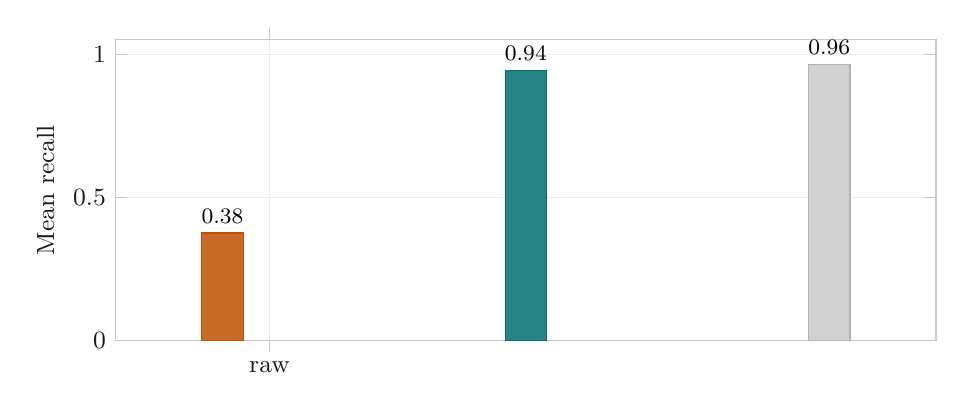
\begin{tikzpicture}
\begin{axis}[ybar,width=12cm,height=5.4cm,bar width=15pt,ymin=0,ymax=1.05,
  ylabel={Mean recall}, symbolic x coords={raw,scaffold,copy ceiling},
  xtick=data, enlarge x limits=0.3, nodes near coords,
  nodes near coords style={font=\footnotesize}]
\addplot[rawstyle] coordinates {(raw,0.375)};
\addplot[scafstyle] coordinates {(scaffold,0.942)};
\addplot[copystyle] coordinates {(copy ceiling,0.964)};
\end{axis}\end{tikzpicture}
\caption{Gemini~3.7~Flash. The scaffold arm (0.942) lands just under the \emph{copy ceiling}
(0.964)---the recall a no-op extractor of the injected context would already achieve. The
$+0.57$ raw$\to$scaffold uplift is almost entirely answer exposure.}
\label{fig:anchor}
\end{figure}

\subsection{Ten models: gain over copy separates them}\label{sec:multi-model}
Table~\ref{tab:sweep} runs the identical paired design across ten models from five providers under
one deterministic configuration. Every model shows a large raw$\to$scaffold uplift
($+0.57$ to $+0.78$) and every model lands just under the copy ceiling: scaffold recall spans
0.897--0.942 against a ceiling of \textbf{0.964} that is a property of the questions and the
injected context---not the model---and is therefore identical across the row. The raw uplift is a
near-constant restatement of exposed gold; it does not separate the models.

The signed \textbf{gain over copy} does. It is negative for all ten (Figure~\ref{fig:gain}), from
$-0.067$ (Gemini~2.5~Flash-Lite) to $-0.022$ (Gemini~3.7~Flash): on this lexical metric no model
recovers gold \emph{beyond} what the exposure check already finds, so they differ only in how much
surfaced gold they \emph{drop}. The ordering is interpretable and tracks recency and capability
rather than provider---the newest, strongest models (Gemini~3.7 and 3.5~Flash, Claude~Haiku~4.5)
sit closest to the ceiling (most faithful restatement), while older or smaller models
(Gemini~2.5~Flash-Lite, GPT-4.1-mini, Mistral-Small-24B) lose measurably more. Two models carried
transport-level truncations under the fixed 2048-token budget (GLM-4.6: 174 truncated, 5 retried;
Gemini~2.5~Flash-Lite: 16 truncated), recorded per row rather than hidden.

\begin{table}[t]\centering\small
\caption{Ten models, one deterministic configuration, $n=510$ (seed 42), sorted by gain over copy
(scaffold recall $-$ copy ceiling). The copy ceiling (0.964) is a property of the questions and
the injected context and is identical across models. The interval shown is the domain-clustered
block bootstrap (the wider, primary one).}
\label{tab:sweep}
\begin{tabular}{lccccc}
\toprule
Model & Raw & Scaffold & Uplift [clustered 95\% CI] & Ceiling & Gain \\
\midrule
Gemini 3.7 Flash      & 0.375 & 0.942 & $+0.567$ $[+0.524,+0.611]$ & 0.964 & \gainneg{-0.022} \\
Gemini 3.5 Flash-Lite & 0.323 & 0.938 & $+0.615$ $[+0.565,+0.667]$ & 0.964 & \gainneg{-0.026} \\
Claude Haiku 4.5      & 0.151 & 0.934 & $+0.783$ $[+0.741,+0.827]$ & 0.964 & \gainneg{-0.031} \\
GLM-4.6               & 0.243 & 0.928 & $+0.685$ $[+0.641,+0.727]$ & 0.964 & \gainneg{-0.036} \\
DeepSeek-Chat         & 0.347 & 0.924 & $+0.578$ $[+0.532,+0.622]$ & 0.964 & \gainneg{-0.040} \\
Llama-3.3-70B         & 0.227 & 0.916 & $+0.688$ $[+0.632,+0.738]$ & 0.964 & \gainneg{-0.049} \\
Qwen-2.5-72B          & 0.309 & 0.914 & $+0.605$ $[+0.562,+0.649]$ & 0.964 & \gainneg{-0.050} \\
Mistral-Small-24B     & 0.285 & 0.906 & $+0.621$ $[+0.558,+0.682]$ & 0.964 & \gainneg{-0.058} \\
GPT-4.1-mini          & 0.162 & 0.905 & $+0.743$ $[+0.697,+0.787]$ & 0.964 & \gainneg{-0.060} \\
Gemini 2.5 Flash-Lite & 0.227 & 0.897 & $+0.670$ $[+0.623,+0.716]$ & 0.964 & \gainneg{-0.067} \\
\bottomrule
\end{tabular}
\end{table}

\begin{figure}[t]\centering
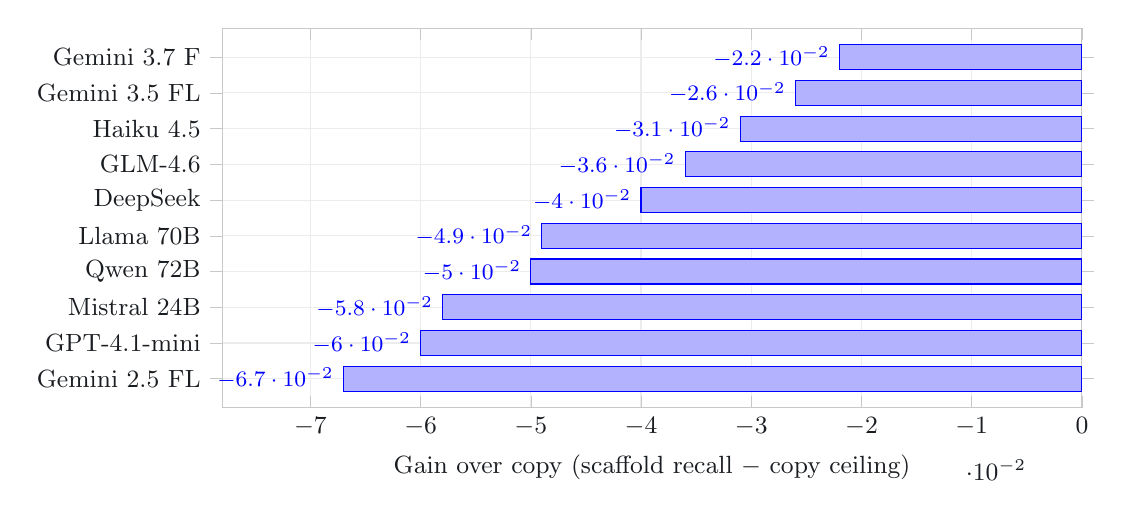
\begin{tikzpicture}
\begin{axis}[xbar,width=12.5cm,height=6.4cm,bar width=9pt,xmin=-0.078,xmax=0,
  xlabel={Gain over copy (scaffold recall $-$ copy ceiling)}, enlarge y limits=0.09,
  symbolic y coords={Gemini 2.5 FL,GPT-4.1-mini,Mistral 24B,Qwen 72B,Llama 70B,DeepSeek,GLM-4.6,Haiku 4.5,Gemini 3.5 FL,Gemini 3.7 F},
  ytick=data, nodes near coords, nodes near coords style={font=\footnotesize},
  every node near coord/.append style={anchor=east},
  every axis plot/.append style={fill=burnt!80,draw=burnt}]
\addplot coordinates {(-0.067,Gemini 2.5 FL) (-0.060,GPT-4.1-mini) (-0.058,Mistral 24B) (-0.050,Qwen 72B) (-0.049,Llama 70B) (-0.040,DeepSeek) (-0.036,GLM-4.6) (-0.031,Haiku 4.5) (-0.026,Gemini 3.5 FL) (-0.022,Gemini 3.7 F)};
\end{axis}\end{tikzpicture}
\caption{Signed gain over copy for all ten models---negative throughout. No model exceeds the copy
ceiling on the lexical metric; the spread ($-0.067$ to $-0.022$) is the axis that separates them
where the near-identical raw uplift does not. Models nearest zero (top) restate the vetted facts
most faithfully.}
\label{fig:gain}
\end{figure}

\subsection{Out-of-domain: the gate prevents jaggedness}\label{sec:ood}
The in-domain result says grounding delivers; the deployment question is whether it \emph{costs}
anything on the general, novel questions a model already handles. On the 60-question out-of-domain
set, judged 0--5 against frontier gold by a cross-family judge across five models, it does not.
Bare and harnessed scores sit near the ceiling in every stratum, and every paired harness$-$bare
delta's 95\% interval includes zero (Table~\ref{tab:ood}): all questions $-0.05$, $[-0.11,0.00]$;
off-domain $-0.09$, $[-0.25,+0.02]$; and even the pre-specified worst case---off-domain questions
on which the gate mis-fired and injected anyway---$-0.23$, $[-0.63,+0.05]$, still spanning zero.

The mechanism is visible in the data. When the gate correctly judges a query off-domain and
\emph{skips} (60 of 100 off-domain gradings), the harnessed answer is identical to bare
($\Delta=+0.00$): with nothing injected there is nothing to distract. The only degradation appears
when the gate over-fires (40 gradings, $\Delta=-0.23$), and it concentrates on the weakest model
(Gemini~2.5~Flash-Lite, $-0.50$) while the stronger models absorb the irrelevant context unharmed.
Confidence-gated injection is thus doing its job: the second axis is met not by models heroically
ignoring bad context, but by the gate mostly not supplying it. We report ``no jaggedness detected''
rather than ``zero effect''---20 questions per stratum and 40 gate-engaged gradings give wide
intervals, so this bounds the regression near zero, it does not prove its absence.

\begin{table}[t]\centering\small
\caption{Out-of-domain non-regression: paired harness$-$bare quality delta (judge 0--5 vs frontier
gold), five models, seeded paired bootstrap 95\% CI. Every interval includes zero. The worst case
is off-domain questions where the confidence gate mis-fired and injected context anyway; the last
row is where it correctly skipped (nothing injected, so identical to bare).}
\label{tab:ood}
\begin{tabular}{lccc}
\toprule
Subset & Mean $\Delta$ & 95\% CI & $n$ pairs \\
\midrule
All general questions              & $-0.05$ & $[-0.11,\ 0.00]$ & 300 \\
\quad adjacent                     & $+0.01$ & $[-0.02,\ 0.05]$ & 100 \\
\quad in-domain-general            & $-0.06$ & $[-0.14,\ 0.00]$ & 100 \\
\quad off-domain                   & $-0.09$ & $[-0.25,\ 0.02]$ & 100 \\
Off-domain, gate mis-fired (worst) & $-0.23$ & $[-0.63,\ 0.05]$ & 40 \\
Off-domain, gate skipped (correct) & $+0.00$ & ---              & 60 \\
\bottomrule
\end{tabular}
\end{table}

% =====================================================================
\section{The Multivariate Bar}\label{sec:multivariate}
In-domain fidelity is one axis of a deployable private-knowledge system, not the whole target.
We state the full bar and where this study sits, so the single number is not mistaken for the
claim.

\begin{enumerate}[topsep=2pt,itemsep=2pt,leftmargin=1.4em]
\item \textbf{In-domain recall / delivery fidelity (this paper).} Excellent, faithful,
attributable recall on questions the curated corpus covers---measured against the copy ceiling so
``faithful'' is quantified, not assumed. Established here across ten models.
\item \textbf{No jaggedness on out-of-domain (established here, \S\ref{sec:ood}).} Injecting
ontology context must not \emph{degrade} the general, novel questions a model already answers well;
irrelevant context is known to distract and to displace correct parametric
knowledge~\cite{shi2023distracted,yoran2024robust,longpre2021entity}. The mitigation is
confidence-gated selective injection---inject in proportion to retrieval score, skip below a
threshold~\cite{mallen2023trust}. On the 60-question out-of-domain set the gated harness holds the
paired quality delta at zero across five models---every 95\% interval includes zero---degrading
only mildly and non-significantly when the gate over-fires, and not at all when it correctly skips.
The gate, not model heroics, is what carries the axis.
\item \textbf{The right baseline is web search, not the bare model (designed).} For an in-domain
question the meaningful comparison is the same model grounded in live web-search results versus
the curated scaffold. The hypothesis is that a vetted, structured corpus is higher-precision and
lower-noise than open-web retrieval~\cite{shi2023distracted}, with the curation cost amortised
once rather than re-paid per query. This is a third grounding arm on the identical question set.
\item \textbf{Attribution (designed).} Every grounded answer already carries its corpus
generation and grounding confidence; a reported attribution-precision metric would close the
loop from ``faithful to the input'' to ``attributable to a named, versioned source.''
\end{enumerate}

\noindent A system that clears all four is the goal: \emph{excellent where it is grounded,
un-degraded where it is not, better than a web search in-domain, and traceable throughout.} The
out-of-domain and web-search arms are multivariate by construction---uplift on the local set and
non-regression on the general set are distinct outcomes that must hold together.

% =====================================================================
\section{Discussion}
\paragraph{What the copy ceiling does and does not say.}
A near-ceiling result does not make grounding worthless---exposing the right facts and having the
model restate them faithfully is exactly what a grounded QA system should do, and the raw arm
shows models cannot do it from parametric memory alone. What the ceiling forbids is the
\emph{inference} that the model is reasoning over ontological structure. For that claim the
evidence is gain over copy, and negative controls (irrelevant, shuffled-target, and label-masked
scaffolds) that we flag as required future work.

\paragraph{Gain over copy as a faithfulness axis.}
Across ten models the gain is uniformly negative ($-0.067$ to $-0.022$): none exceeds the copy
ceiling, so on this lexical metric no model demonstrably recovers gold beyond what its injected
context already exposes---the behaviour is faithful extraction, not inference over structure. The
spread is small but ordered, and it tracks recency and capability rather than provider: the newest
Gemini models and Claude~Haiku~4.5 restate the surfaced facts most completely (gain nearest zero),
while older or smaller models drop more of what they were shown. For a private-knowledge system
this is the operative quality signal---not ``does grounding help'' (it always does, and hugely)
but ``how faithfully does this model deliver the vetted facts''---and the copy ceiling is what lets
that be read off directly rather than inferred from an uplift that mostly measures exposure.

\paragraph{Two axes, held together.} The deployment claim is conjunctive: a private-knowledge
system must deliver in-domain \emph{and} not regress out-of-domain, and the two are measured on
different instruments---lexical recall against a copy ceiling, and judged quality against frontier
gold. Both hold here: near-ceiling in-domain delivery across ten models, and no detected jaggedness
across five, carried by the confidence gate declining to inject when it judges a query
out-of-domain. That conjunction is the property a single in-domain number cannot establish. What
remains to close the bar is the right \emph{baseline}---the same model grounded in a web search
rather than the bare model---and an attribution-precision metric; both are specified in
\S\ref{sec:multivariate} and neither is measured here.

% =====================================================================
\section{Limitations and Threats to Validity}\label{sec:limits}
\begin{itemize}[topsep=2pt,itemsep=1pt]
\item \textbf{Estimand.} The primary metric is \emph{lexical gold-title recall}: it counts whether
expected titles appear, not relation direction, negation, correctness of explanation, or
contradiction. ``Grounding'' should be reserved for a composite that also checks these.
\item \textbf{Leakage is deliberate.} Questions, gold and scaffold derive from one graph; the copy
ceiling measures the leakage rather than removing it. Absolute recall is a lower bound (lexical
matching under-counts paraphrase), possibly arm-dependently.
\item \textbf{Single sample.} One completion per arm; at \texttt{temperature}=0 this is
deterministic but leaves no estimate of a model's own sampling variance. Convergence claims need
replicates and a pre-registered equivalence margin.
\item \textbf{Non-independence.} Multiple questions share a class/domain; we report a
domain-clustered interval but 15 domains is a small cluster count, so domain-level generalisation
is uncertain.
\item \textbf{Out-of-domain arm is near-ceiling and small.} The jaggedness test uses judged 0--5
quality on 60 general questions (20 per stratum, five models); bare scores already sit near~5, so it
bounds \emph{regression} near zero rather than demonstrating \emph{help}, and the wide intervals
(40 gate-engaged gradings) warrant ``no jaggedness detected,'' not proof of no effect. Gold and
judge are single frontier models; cross-family judging mitigates but does not eliminate judge bias.
\item \textbf{Population.} Eligibility filters (dense, well-defined classes) select cases
favourable to grounding; sparse classes, aliases, ambiguous phrasing, multi-hop and off-ontology
queries are untested. Prompts name canonical titles, easing retrieval.
\item \textbf{Single graph, single domain family.} Fidelity to one curated Web3/XR/AI ontology;
generalisation to other graphs is plausible but unshown. The corpus is AI-generated synthetic
content produced under human direction---an ontology testbed, not an authoritative encyclopaedia.
\end{itemize}

% =====================================================================
\section{Conclusion}
Ontology-scaffold grounding produces a large recall uplift for every model
tested, tight under a domain-clustered bootstrap---but on the strongest model that uplift is, to
within measurement, exactly what a copy of the injected context would score. The honest quantity is not the uplift but the \emph{gain over
copy}, and across all ten models tested it is small and uniformly negative ($-0.067$ to
$-0.022$)---the axis that separates them where the near-identical raw uplift cannot. Grounding
evaluations that inject graph-derived gold should report a copy ceiling as standard. We release the harness, the frozen seed-42 question set, and all per-row artefacts.

\paragraph{Reproducibility.} Harness, sweep drivers and per-row outputs:
\texttt{github.com/DreamLab-AI/loom} (\texttt{bench/}). Every run ships its honesty notes and its
copy ceiling.

\printbibliography

\end{document}
